% Proposal layout based on the supplied example; example research content omitted.
\documentclass[a4paper,12pt]{article}
\usepackage[T1]{fontenc}
\usepackage[utf8]{inputenc}
\usepackage[left=3cm,right=3cm,top=2cm,bottom=2cm]{geometry}
\usepackage{graphicx}
\usepackage{tabularx}
\usepackage{parskip}
\usepackage[authoryear,round]{natbib}
\usepackage{url}
\usepackage{acronym}

% Keep figures and tables in source order. Each block moves intact to the next
% page when needed, while retaining standard captions, numbering, and labels.
\makeatletter
\newenvironment{placedfigure}
  {\par\addvspace{\intextsep}\noindent\begin{minipage}{\linewidth}\def\@captype{figure}}
  {\end{minipage}\par\addvspace{\intextsep}}
\newenvironment{placedtable}
  {\par\addvspace{\intextsep}\noindent\begin{minipage}{\linewidth}\def\@captype{table}}
  {\end{minipage}\par\addvspace{\intextsep}}
\makeatother

% Acronyms expand on first use; plural forms share the singular's usage state.
\acrodef{LCM}{land cover map}
\acrodefplural{LCM}[LCMs]{land cover maps}
\acrodef{SOTA}{state-of-the-art}
\acrodef{LCC}{land cover classification}
\acrodef{GFM}{geospatial foundation model}
\acrodefplural{GFM}[GFMs]{geospatial foundation models}
\acrodef{LULC}{land use and land cover}
\acrodef{NDVI}{normalized difference vegetation index}
\acrodef{DEM}{digital elevation model}
\acrodef{ViT}{vision transformer}

\title{A Solid Foundation? Geospatial Foundation Models for Land Cover Mapping in Africa}
\author{Tomer Adam Peled}
\date{31 October 2026}

\begin{document}
\begin{titlepage}
  \centering
  \vspace*{1.5cm}
  {\LARGE\bfseries A Solid Foundation? Geospatial Foundation Models for Land Cover Mapping in Africa\par}
  \vspace{1cm}
  {\Large\itshape Master Thesis Proposal\par}
  \vspace{1cm}
  {\large Tomer Adam Peled\par}
  \vspace{0.5cm}
  {\large 31 October 2026\par}
  \vspace{1cm}
  {\large Main supervisor: Dainius Masiliunas\par}
  {\large Secondary supervisor: Nandika Tsendbazar\par}
  \vfill
  
\includegraphics[width=7cm]{title/WUR_RGB_standard-eps-converted-to.pdf}\par
  \vspace{1cm}
  {\large Wageningen University \& Research\par}
  {\large Laboratory of Geo-Information Science and Remote Sensing\par}
  \vspace*{2.5cm}
\end{titlepage}

\tableofcontents
\clearpage

\section{Context and Background}
Accurate \acp{LCM} are essential for a large variety of use cases. For example, \acp{LCM} contribute directly to the monitoring of multiple targets of the United Nations' Sustainable Development Goals, such as protecting and restoring ecosystems, enhancing inclusive and sustainable urbanization, combating deforestation and desertification, and monitoring carbon stocks \citep{moraMonitoringProgressSustainable2016}. But while the current \ac{SOTA} \acp{LCM} have a respectable overall accuracy, the accuracy in certain regions and for certain classes can be poor \citep{xuComparativeValidationRecent2024,zhaoAssessingAccuracyConsistency2023}. Regions with a more heterogeneous landscape, such as Oceania and subsaharan-Africa, have worse classification accuracy compared to homogeneous regions such as Europe \citep{zhaoAssessingAccuracyConsistency2023}. Heterogeneous landscapes require more spatial detail for correct classification, and suffer more from problems such as reference data uncertainty \citep{xuComparativeValidationRecent2024}. Classes such as 'Crops' and 'Built-up' also have lower accuracy compared to more common classes such as 'Water', 'Trees', and 'Bare Ground' \citep{xuComparativeValidationRecent2024}. These poorly-classified classes often exhibit similar spectral profiles to other classes (e.g. cropland, grassland, and shrubland looking similar).  The classification accuracy of these classes within heterogeneous regions is often particularly poor. For example, \citet{tsendbazarProductValidationReport2022} found that the 'Built-Up' class in the WorldCover map \citep{zanagaESAWorldCover102022} has a users' accuracy of 47.1\% in Africa, compared to 65.9\% globally. Similarly, cropland has a producers' accuracy of 79.3\% globally, but just 58.9\% in Africa. Critically, accurate mapping of these regions and classes is especially important for various applications. \citet{bettencourtInfrastructureDeficitsInformal2025} show that urban land cover is systematically associated with human development indicators, and \citet{kernerHowAccurateAre2024a} show that inaccuracies in cropland coverage can produce misleading agricultural statistics and estimates. Improving \ac{LCC} in Africa, especially accurate classification of the built-up and cropland classes, is therefore an important and significant goal.

\ac{LCC} lends itself naturally to utilizing multi-modal data. Multi-modality refers to using multiple different sources of information, or modalities, as model input (e.g. using both optical and radar data). Multi-modality is useful for \ac{LCC} because different modalities show different properties of the underlying land-cover, and can therefore help distinguish between classes that might appear similar in other modalities \citep{joshiReviewApplicationOptical2016}. For example, radar data can give information on the texture and wetness of the ground, which is not knowable from optical images. This information could be relevant for distinguishing between different classes. Furthermore, different modalities can 'compensate' for weaknesses in other modalities, such as radar being able to penetrate cloud cover which blocks optical light. Combining different modalities has successfully been used for \ac{LCC} in many studies \citep{joshiReviewApplicationOptical2016}.
For example, \citet{mahlasiEcologicalMappingGeospatial2026} show that a model with Sentinel-1, \ac{NDVI}, and \ac{DEM} as input modalities outperformed unimodal models at separating peatland from other vegetation, and \citet{shanduEnhancingLandCover2026} show that combining Sentinel-2 and \ac{DEM} data raised model accuracy by about 6 points and reduced ambiguity for minority classes compared to purely Sentinel-2 based model. Global \acp{LCM} such as WorldCover \citep{zanagaESAWorldCover102022} and its successor 'Copernicus Global Land Cover and Tropical Forest Mapping and Monitoring Service' \citep{JRC2026ATBDLCM10} successfully combine multiple modalities such as optical, radar, elevation, and climate data for their products.

Another way to potentially improve \ac{LCC} is via utilizing temporal information. Multi-temporality refers to using multiple different images of the same location taken at different times, as opposed to using a single (time-averaged) image. One way temporal information can improve \ac{LCC} is by providing insight into the phenology of the underlying vegetation, which can help separate classes which are otherwise similar but have different temporal behavior (e.g. crop, herbaceous vegetation, and shrubs) \citep{mullerMiningDenseLandsat2015}. Multi-temporal data has been used for \ac{LCC} in previous studies. \citet{lopesImprovingAccuracyLand2020} used optical and radar time-series to improve \ac{LCC} accuracy in cloud covered regions. \citet{griffithsIntraannualReflectanceComposites2019} compared various time-averaging strategies, and found that using shorter time-series intervals improved overall accuracy, especially for highly dynamic classes. \citet{vuoloHowMuchDoes2018} compared multi-date and single date Sentinel-2 data for crop type classification, and concluded that multi-date data is much more effective when the optimal single-date measurement time isn't known beforehand. \citet{xuComparativeValidationRecent2024}, a comparison of various 10m-resolution \ac{LULC} maps, advices map-makers to include multi-temporality to help separate classes that are hard to characterize.

A promising new way to potentially more effectively use the full range of available modalities and temporal information for \ac{LCC} is by utilizing \acp{GFM} \citep{yangSurveyMultimodalGeospatial2025}. \acp{GFM} are a type of deep learning models which have been 'pretrained' on large and diverse earth observation datasets. Pretraining is done in a self-supervised way, eliminating the need for manually-created labels during the pretraining process. The most common self-supervised training technique is 'masking': part of the input earth observation data is covered up (masked), and the models are then tasked with recreating the masked out area as accurately as possible. This pretraining process aims to train the model to create generalized geospatial representations. These representations can then be fed to a simple 'decoder' model, which can then be trained for various downstream tasks, such as land-cover mapping \citep{tuiaArtificialIntelligenceAdvance2025}. The expectation is that \acp{GFM} are able to extract information from the input modalities and temporal data better than a non-pretrained model can.

\section{Research Needs}
\acp{GFM} are quite new, and the evidence of their effectiveness is mixed: using \acp{GFM} does not consistently improve classification performance. \citet{marsocciPANGAEAGlobalInclusive2025}, comparing models across 11 datasets, have found the baseline U-net and \ac{ViT}-models to achieve comparable results to \acp{GFM} when trained with the full labelled datasets. \acp{GFM} did become more competitive with limited data labels. Using \acp{GFM} with multiple modalities also achieves mixed results. \citet{schindleggerNowWeKnow2026} have found that using Sentinel-1 and Sentinel-2 data did not significantly improve classification performance as compared to using just Sentinel-2 data when evaluating the \acp{GFM} TerraMind \citep{jakubikTerraMindLargeScaleGenerative2026} and THOR \citep{forgaardTHORVersatileFoundation2026} on two datasets. The authors attribute this to the models' relatively simple modality fusion mechanisms, which might not sufficiently extract complementary information from the modalities. \citet{simumbaGEOBench2PerformanceCapability2026} compared \ac{GFM} performance across 19 datasets, and found that no single \ac{GFM} dominates, with performance being strongly influenced by the relevancy of the pretraining of the \ac{GFM} to the individual task.

At the same time, \acp{GFM} have been found to achieve better accuracy than 'specialist' models for minority classes and harder to classify regions. The \ac{GFM} Presto \citep{tsengLightweightPretrainedTransformers2024} has been able to outperform specialist models on crop-type classification tasks \citep{butskoDeployingGeospatialFoundation2025a}, especially for under-represented classes as well as mapping in more challenging regions. \citet{ballGeospatialFoundationModels2026} have similarly found that \acp{GFM} outperformed traditional models on tree species mapping, with the most important benefits arising from identifying minority species more accurately.

It remains to be researched whether a \ac{GFM}, used with multiple modalities and temporal information, can achieve better accuracy than specialist models for \ac{LCC} in Africa for challenging classes such as built-up or cropland, and in heterogeneous regions. The current literature suggests that utilizing a \ac{GFM} for this use-case could be beneficial, especially if a \ac{GFM} with relevant pretraining is used. Improving \ac{LCC} accuracy for these classes could result in better \acp{LCM} for Africa, which would directly contribute to many projects.

Furthermore, the effect of including various modalities and temporal information on \ac{LCC} accuracy with \acp{GFM} is unknown. Knowing the importance of modalities and temporalities would allow future projects to focus resources on the most helpful ones, or investigate why some modalities or temporalities don't increase accuracy as much as might be expected.

\section{Overall Research Objectives and Research Questions}

\subsection{Research Objective}

\acp{GFM} might already be capable of outperforming specialist models for \ac{LCC} accuracy for challenging classes in Africa. The first research objective is to learn whether the \ac{GFM} Galileo is capable of this. Furthermore, it would be valuable to know which input modalities and/or temporalities are most valuable for \ac{LCC} accuracy. The second goal is to understand the effect of different modalities and/or temporalities on \ac{LCC} accuracy.

\subsection{Research Questions}
\begin{enumerate}
  \item How does Galileos' \ac{LCC} accuracy compare to existing models for \ac{LCC} in Africa?
  \item How does the addition or removal of different modalities and temporal information affect Galileo performance for \ac{LCC} in Africa?
        \begin{enumerate}
          \renewcommand{\labelenumii}{\alph{enumii}.}
          \item How does the addition or removal of sentinel-1, sentinel-2, or \ac{DEM} data change Galileo performance for \ac{LCC} in Africa?
          \item How does using a yearly vs. monthly Sentinel-1 or Sentinel-2 composite change Galileo performance for \ac{LCC} in Africa?
        \end{enumerate}
\end{enumerate}

\section{Methodology}
This section describes the target and testing datasets. It further describes the \ac{GFM} Galileo, the input datasets for the model,  preliminary tests for deciding on important model configurations, and consequent model training for answering the research question. Finally the model evaluation, model comparison, and map accuracy assessment strategies are described. See Figures~\ref{fig:methodology-experiments} and~\ref{fig:methodology-evaluation} for flowcharts summarizing the process.


\begin{placedfigure}
  \centering
  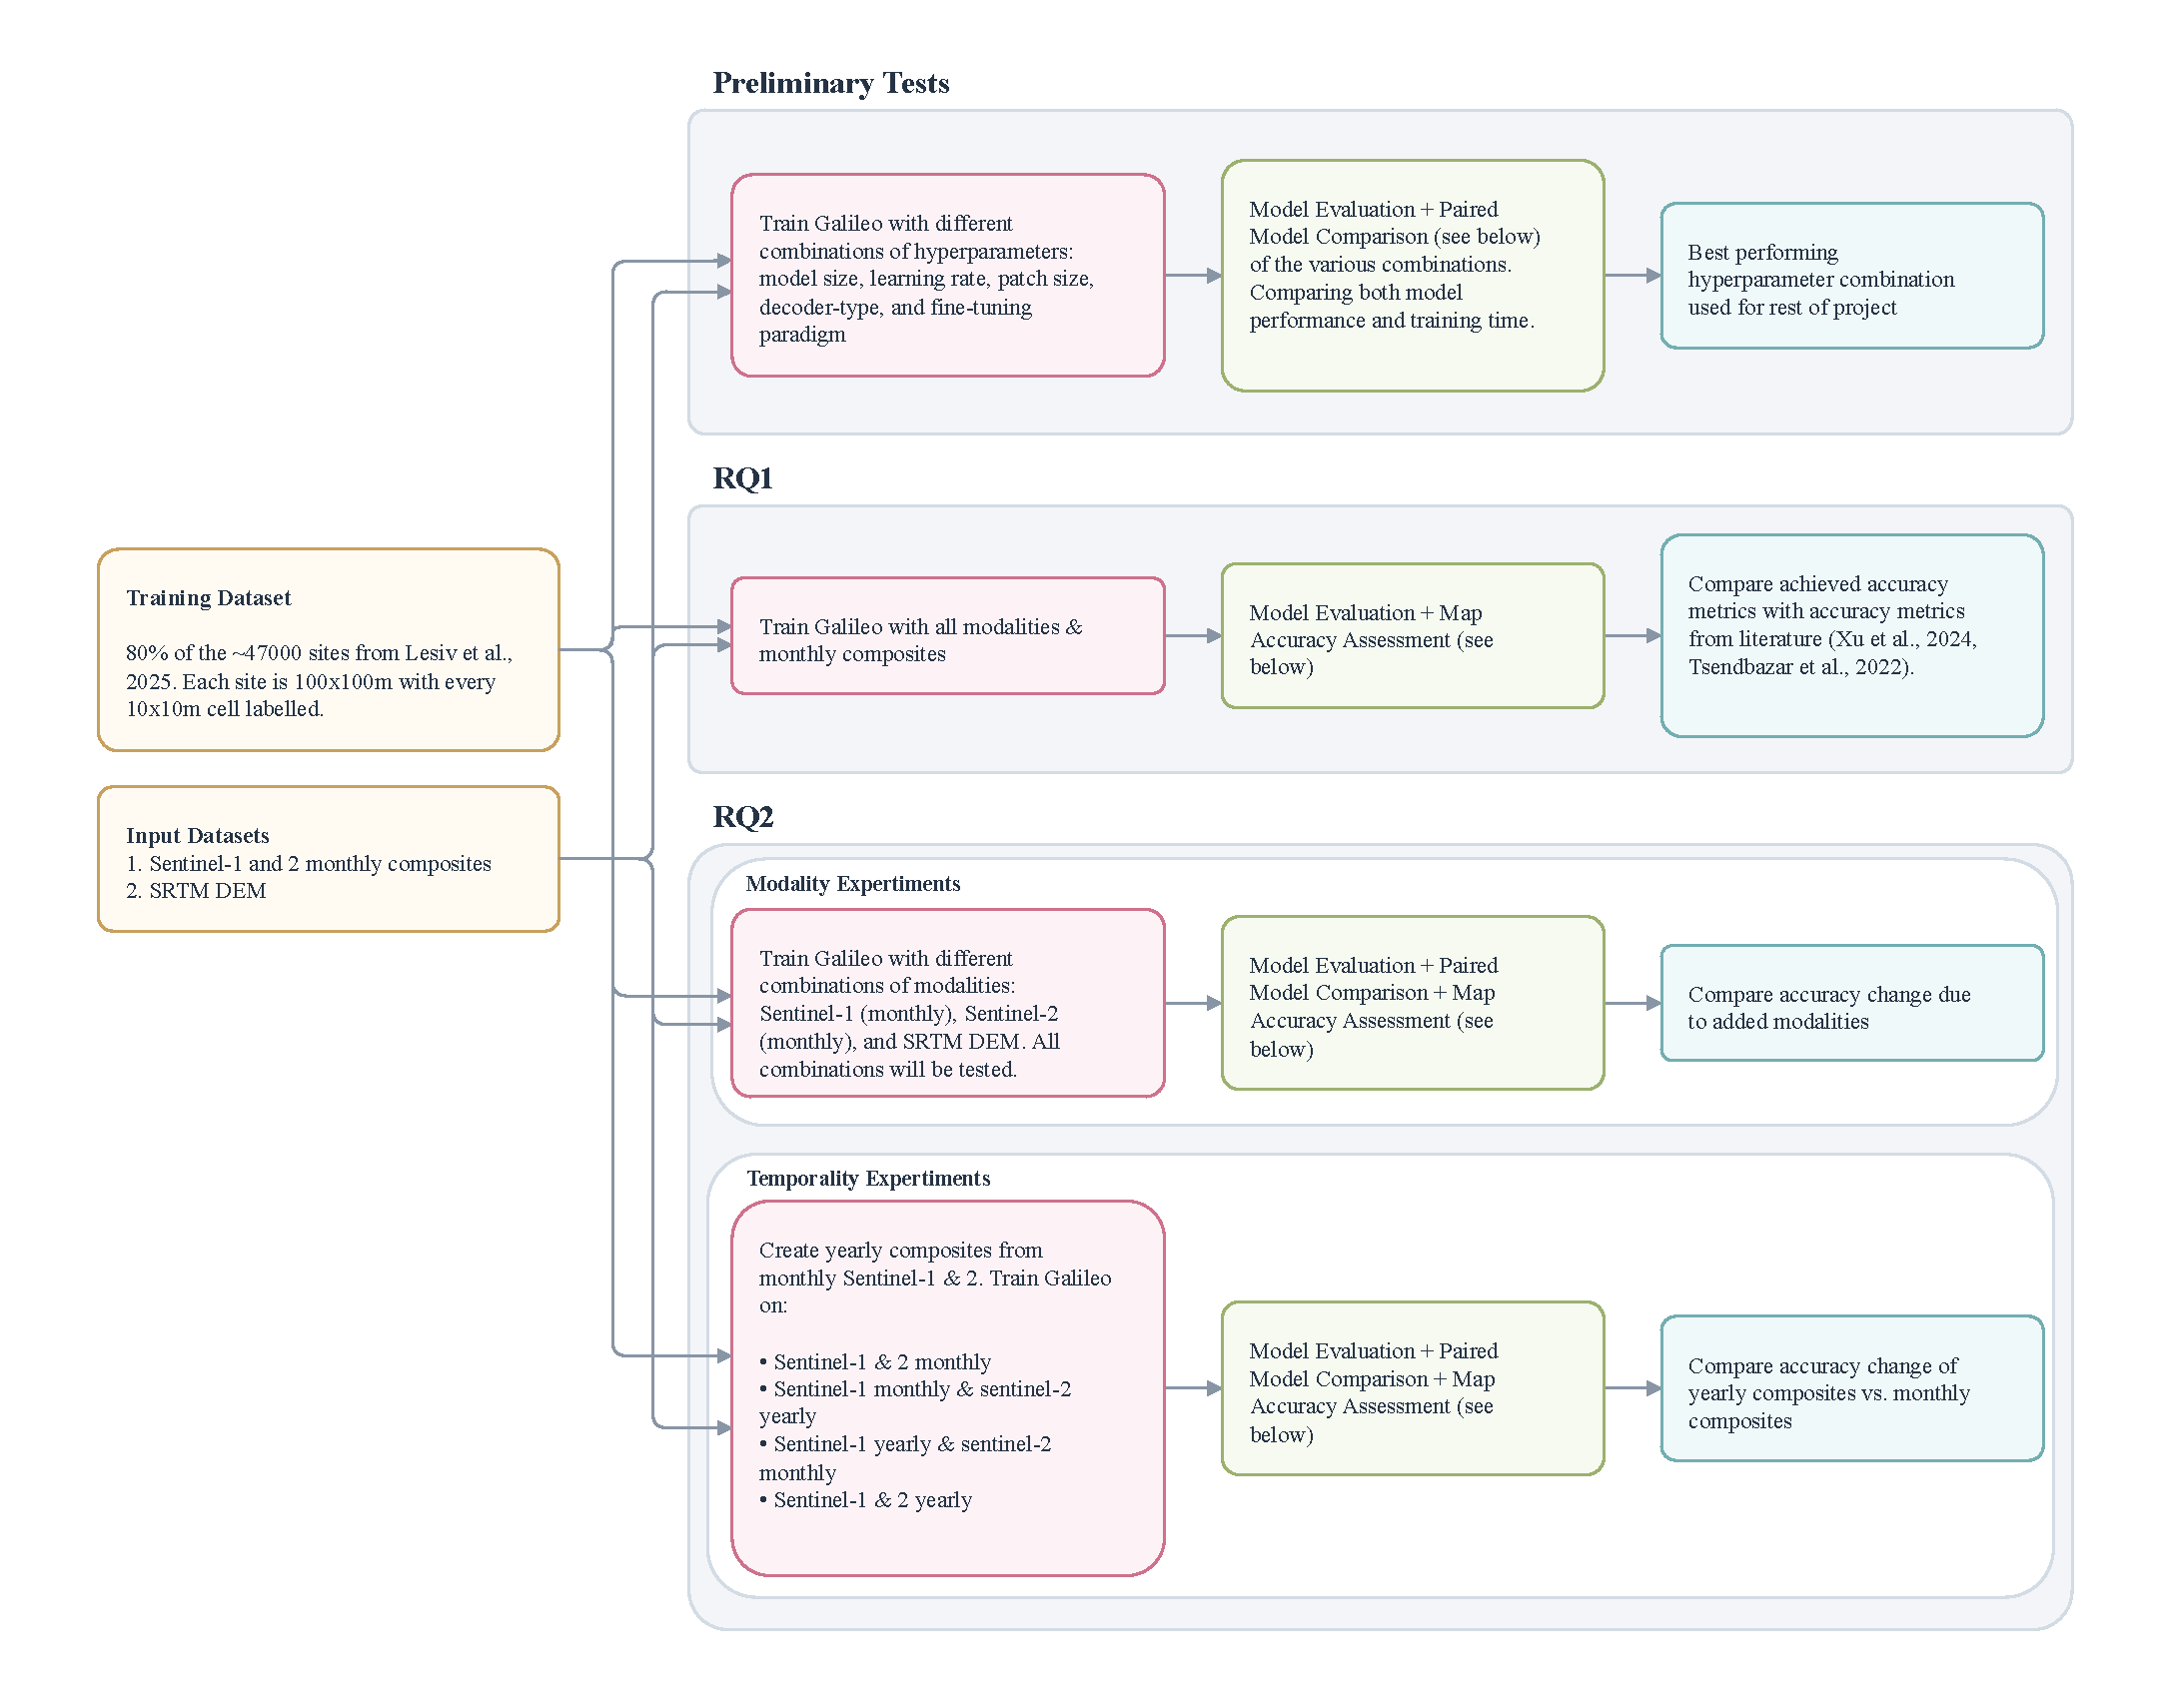
\includegraphics[width=\textwidth,height=0.82\textheight,keepaspectratio]{img/methodology_flowchart_01.pdf}
  \caption{Overview of the preliminary experiments and the experiments for the two research questions.}
  \label{fig:methodology-experiments}
\end{placedfigure}
\begin{placedfigure}
  \centering
  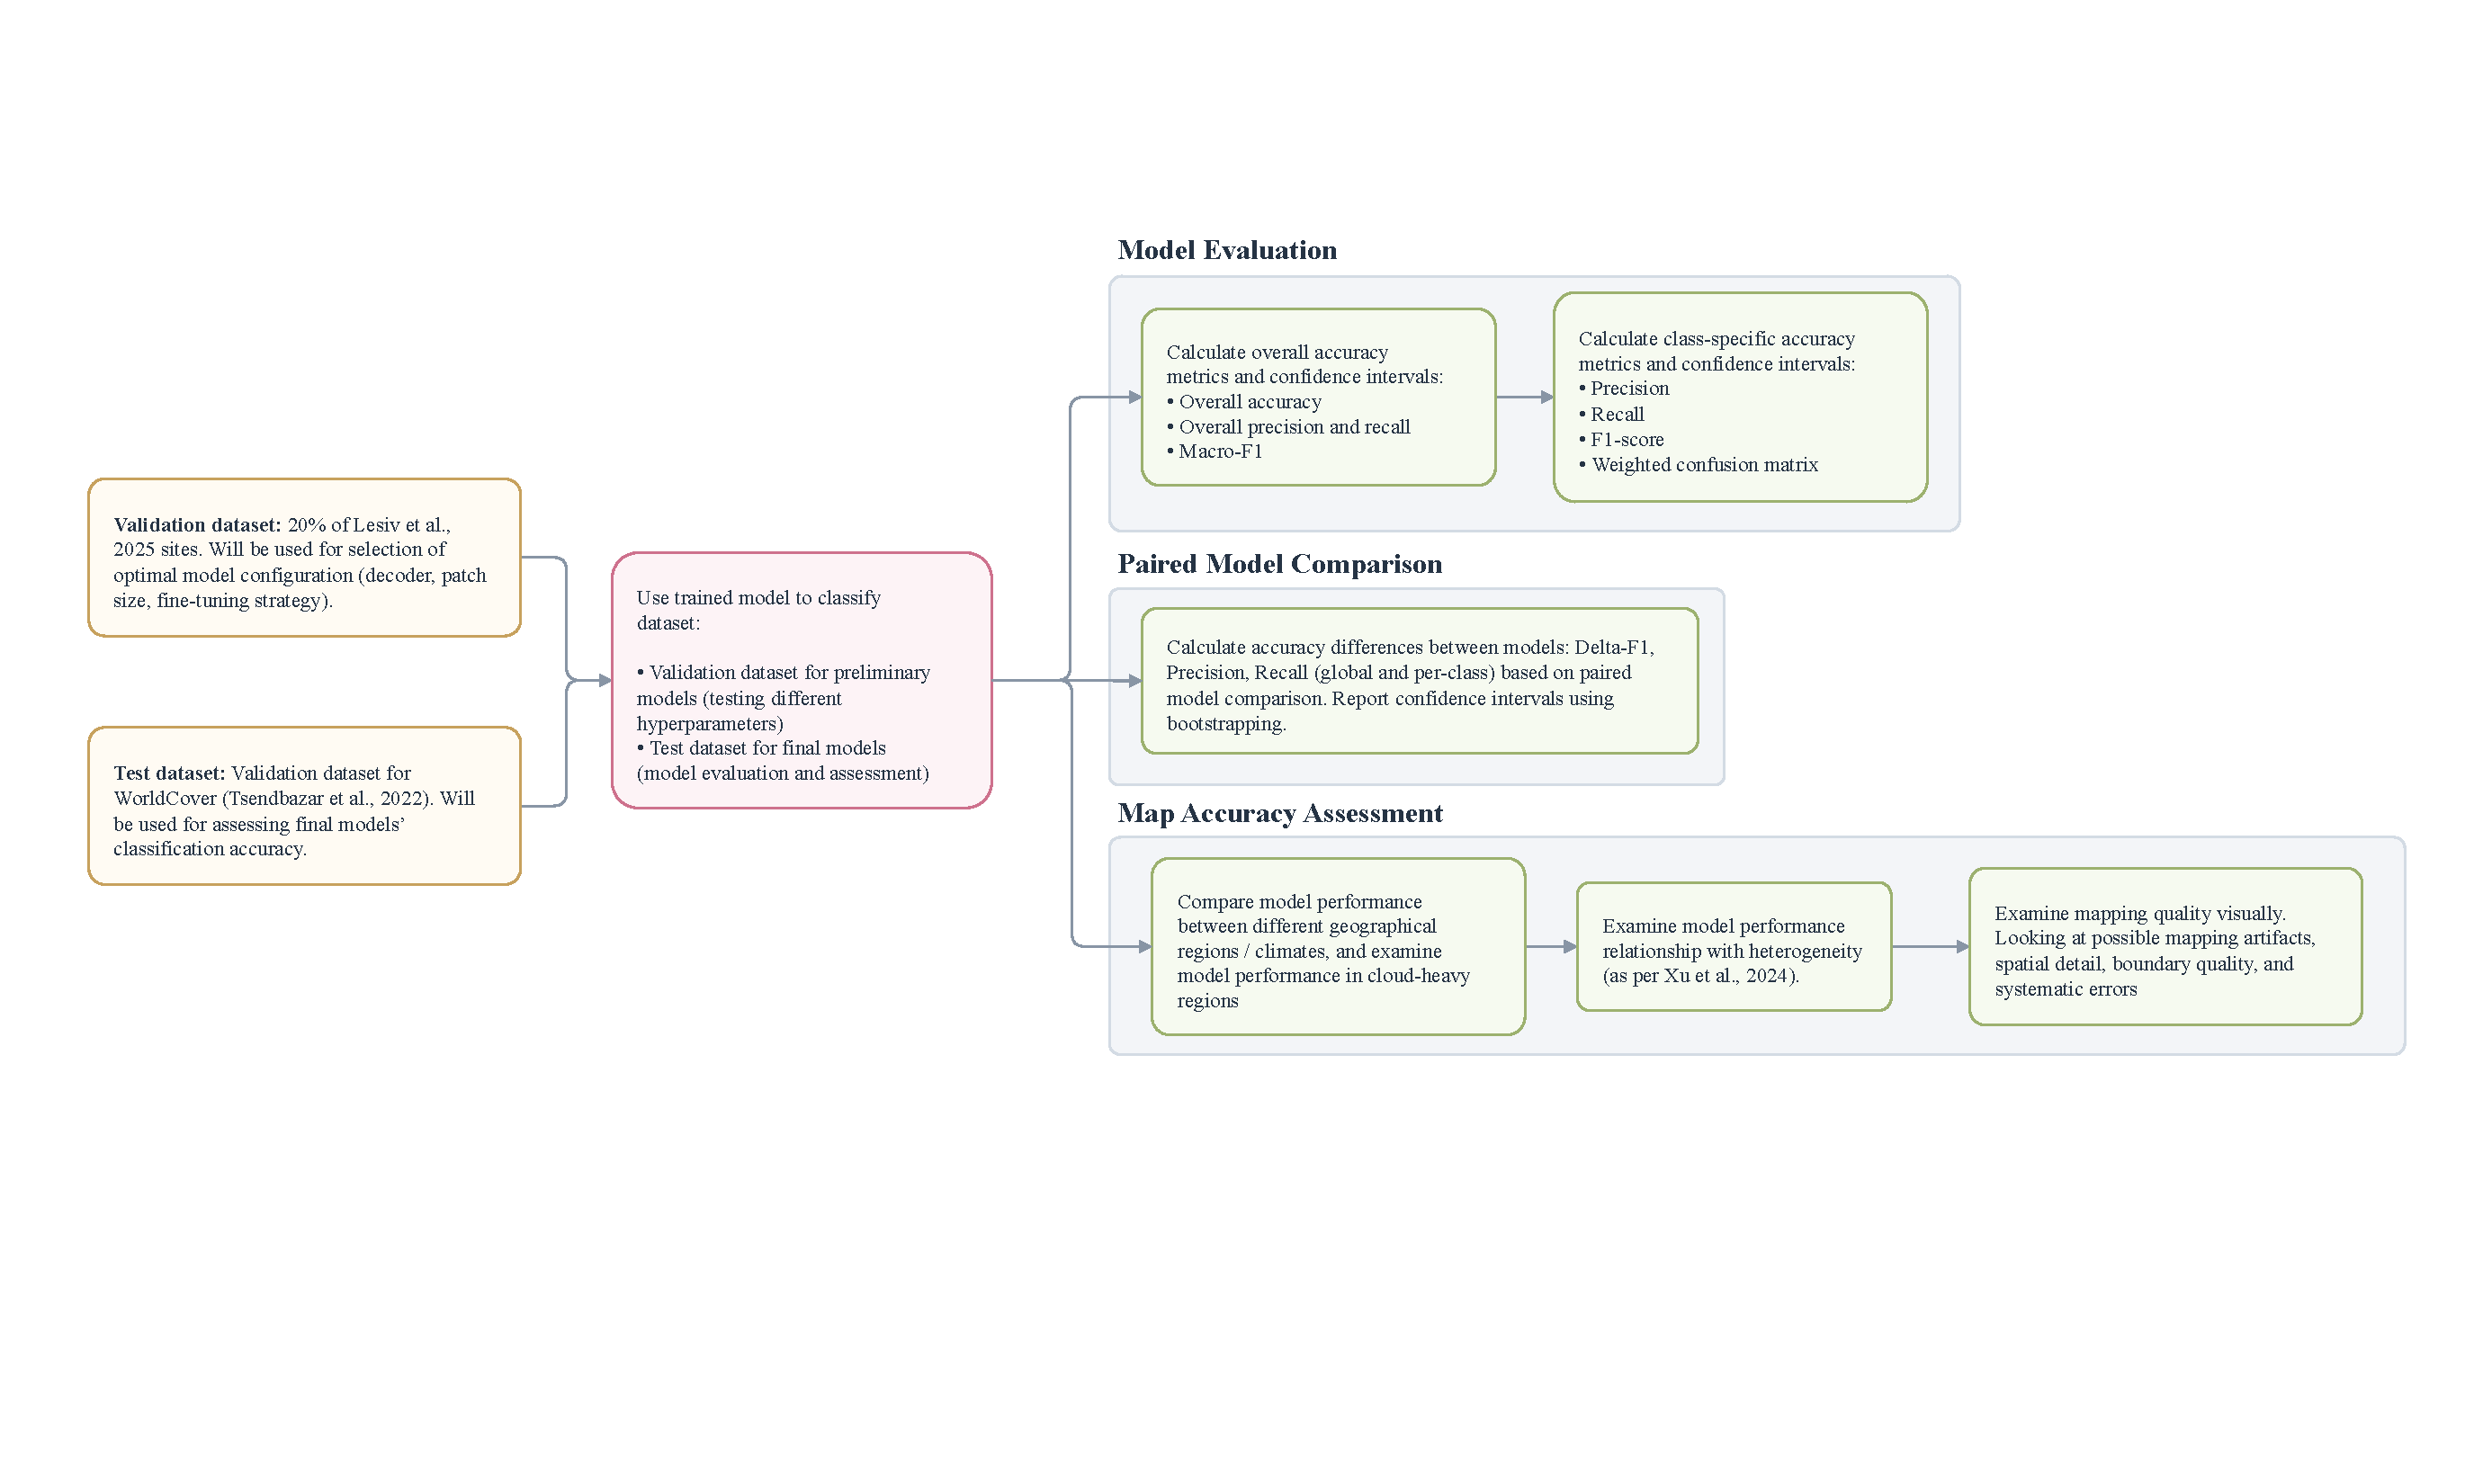
\includegraphics[width=\textwidth,height=0.82\textheight,keepaspectratio]{img/methodology_flowchart_02.pdf}
  \caption{Overview of model evaluation, paired model comparison, and map accuracy assessment.}
  \label{fig:methodology-evaluation}
\end{placedfigure}

\subsection{Target \& Testing Datasets}
\subsubsection{Target Dataset}
This thesis will use a reference land-cover dataset created by \citet{lesivGlobalReferenceData2025}. The dataset consists of approximately 165,000 sites, distributed worldwide. Each site is 100x100m, subdivided into 10x10m cell (Figure~\ref{fig:geowiki-site}). Each cell has been labelled by a team of IIASA experts using GeoWiki, a website for manual land-cover labelling through visual interpretation of satellite images. As this thesis will focus on Africa, only sites located in Africa will be used, reducing the amount of sites to 44,644. The land-cover dataset includes sites distributed all over the continent (Figure~\ref{fig:geowiki-africa-sites}), and contains the classes 'Bare Ground', 'Crops', 'Herbaceous Vegetation', 'Shrubs', 'Trees', 'Built-up', and 'Water'. The dataset classes are imbalanced, with grassland, shrub, and trees dominating (Figure~\ref{fig:geowiki-class-balance}).

\begin{placedfigure}
  \centering
  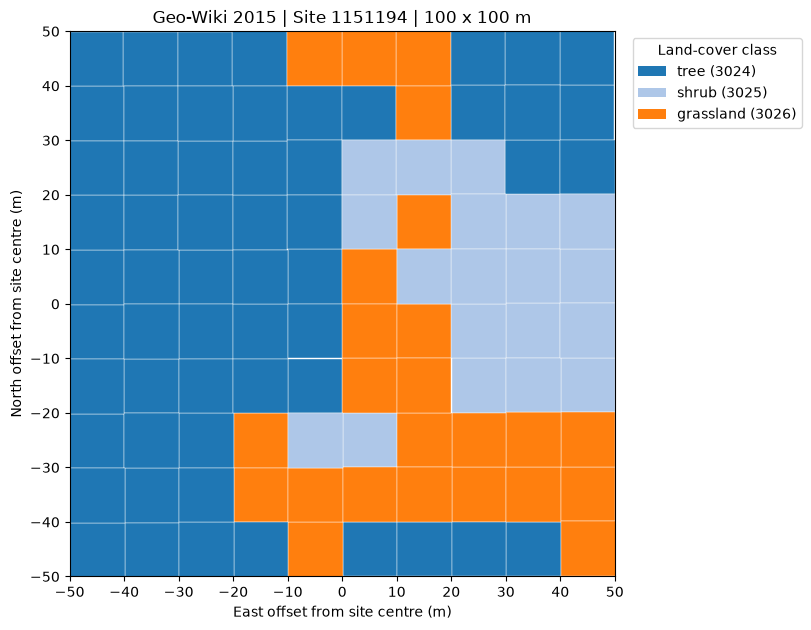
\includegraphics[width=\textwidth,height=0.82\textheight,keepaspectratio]{img/geowiki-2015-example-site.png}
  \caption{Example Geo-Wiki 2015 reference site (site 1151194), showing land-cover labels in a 100 by 100 m site divided into 10 by 10 m cells.}
  \label{fig:geowiki-site}
\end{placedfigure}

\begin{placedfigure}
  \centering
  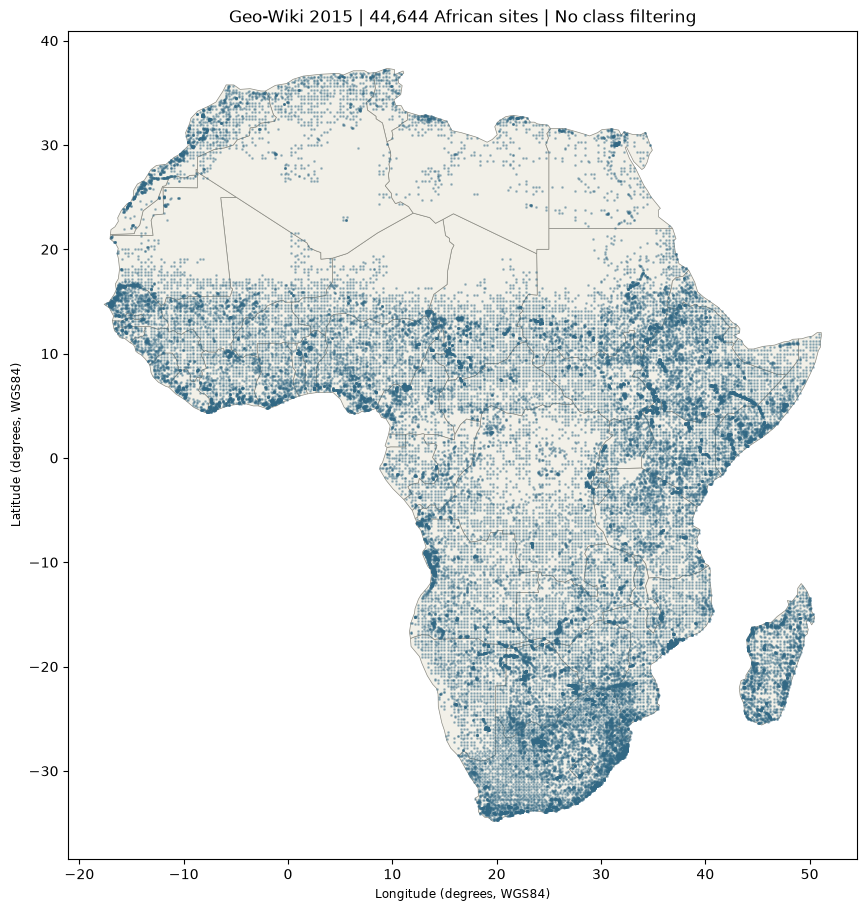
\includegraphics[width=\textwidth,height=0.82\textheight,keepaspectratio]{img/geowiki-2015-africa-site-distribution.png}
  \caption{Distribution of the 44,644 African Geo-Wiki 2015 sites.}
  \label{fig:geowiki-africa-sites}
\end{placedfigure}

\begin{placedfigure}
  \centering
  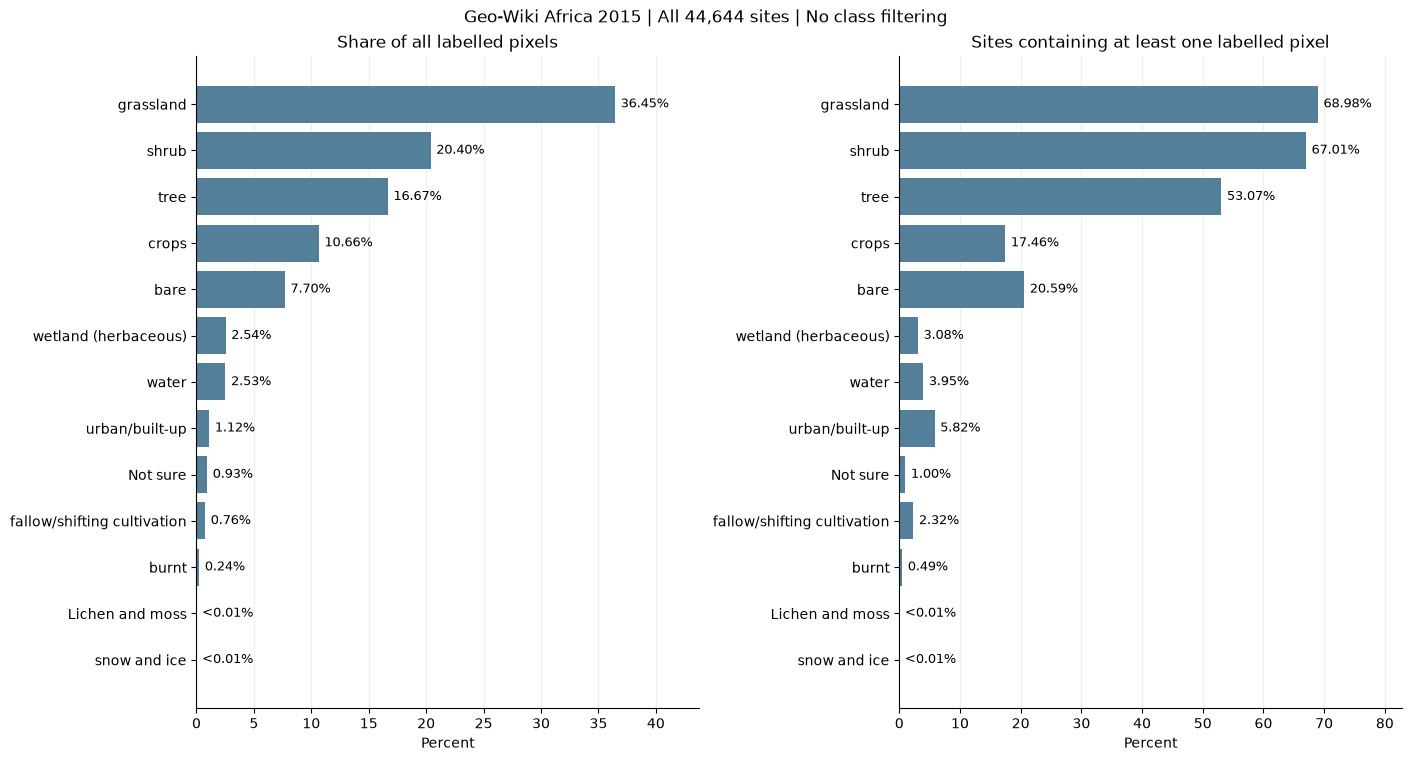
\includegraphics[width=\textwidth,height=0.82\textheight,keepaspectratio]{img/geowiki-2015-africa-class-balance.png}
  \caption{Class balance across all 44,644 African Geo-Wiki 2015 sites: share of labelled pixels (left) and share of sites containing each class (right).}
  \label{fig:geowiki-class-balance}
\end{placedfigure}

A validation dataset will be created from the \citet{lesivGlobalReferenceData2025} using 20\% of the sites. Of the remaining 80\%, a subsample will be used for as the training dataset. Proportional sampling based on class occurrence with a minimum amount of samples for each class will be applied \citep{zhuOptimizingSelectionTraining2016}. Proportional sampling with a minimum amount of samples for each class provides a balanced alternative between proportional sampling, which might not provide enough training samples for minority classes, and equal sampling, which might cause the model to overpredict minority classes. The minimum amount of samples per class will be decided on at a later date. Subsampling will be applied to decrease the amount of download and processing time required, as well as to improve the class balance of the dataset. If achievable within the projects' allocated time and compuational resources, the full 80\% of the dataset will be used instead.

\subsubsection{Testing Dataset}
The dataset created by \citet{tsendbazarProductValidationReport2022} will be used as the independent testing dataset. This dataset has been created to validate the WorldCover \citep{zanagaESAWorldCover102022} map, and has 21,624 global sites, of which 3,599 are in Africa. The dataset is organized in the same way as \citet{lesivGlobalReferenceData2025}: each 100x100m site is split up into 10x10m cells, with the land-cover of each cell having been manually labelled by experts. This dataset will only be used to assess the accuracy of the final models. (Not actually sure about using this dataset for testing -> Might be a problem for urban specifically. Other option is to create a test dataset from the Lesiv et al. data)

\subsection{Galileo}
Galileo \citep{tsengGalileoLearningGlobal2025} was chosen as the base \ac{GFM} for this research. Galileo has been trained with relevant input modalities for \ac{LCC}: Sentinel-1, Sentinel-2, and \ac{DEM}. Furthermore, it was trained with multi-temporal data, namely monthly sentinel-1 and 2 time-series. Other \acp{GFM}, such as TerraMind \citep{jakubikTerraMindLargeScaleGenerative2026}, THOR \citep{forgaardTHORVersatileFoundation2026}, and Prithvi \citep{szwarcmanPrithviEO20VersatileMultiTemporal2026} were considered, but either did not support multi-temporal data (in the case of TerraMind and THOR), or did not support multiple modalities (in the case of Prithvi). The \acp{GFM} Presto \citep{tsengLightweightPretrainedTransformers2024} and AnySat \citep{astrucAnySatOneEarth2025} do support both multi-modal and multi-temporal data, but Presto works on a pixel-by-pixel basis and does not utilize spatial context, and AnySat has not been pretrained with standalone DEM-data, and has been trained on less globally well-distributed training data.

Galileo has been pretrained on a global dataset spanning 127,155 sites, each site being 960x960m (96x96 pixels) and consisting of various input datasets with different temporal resolutions (Table~\ref{tab:galileo-inputs}). Pretraining was performed using masking, applied either at pixel-level or at patch-level.

\begin{placedtable}
  \centering
  \caption{Input datasets and temporal resolutions used in Galileo pretraining \citep{tsengGalileoLearningGlobal2025}.}
  \label{tab:galileo-inputs}
  \small
  \begin{tabularx}{\textwidth}{@{}>{\raggedright\arraybackslash}p{0.21\textwidth} >{\raggedright\arraybackslash}X >{\raggedright\arraybackslash}p{0.22\textwidth}@{}}
    \hline
    \textbf{Modality}      & \textbf{Inputs}                                                               & \textbf{Temporal Resolution}    \\
    \hline
    Sentinel-1 SAR         & VV, VH (2 bands)                                                              & Monthly                         \\[0.4em]
    Sentinel-2 MSI         & B2, B3, B4, B5, B6, B7, B8, B8A, B11, B12 (10 bands)                          & Monthly                         \\[0.4em]
    Sentinel-2 \ac{NDVI}   & \ac{NDVI} derived from B8 and B4 (1 band)                                     & Monthly                         \\[0.4em]
    SRTM \ac{DEM}          & Elevation, slope (2 bands)                                                    & Static                          \\[0.4em]
    Dynamic World          & Nine land-cover class probabilities                                           & Spatial, aggregated across time \\[0.4em]
    WorldCereal            & Five crop-related mapping layers                                              & Spatial, aggregated across time \\[0.4em]
    ERA5                   & 2 m temperature, total precipitation (2 variables)                            & Monthly time series             \\[0.4em]
    TerraClimate           & Climate water deficit, soil moisture, actual evapotranspiration (3 variables) & Monthly time series             \\[0.4em]
    VIIRS nighttime lights & Average radiance (1 variable)                                                 & Time series                     \\[0.4em]
    LandScan and location  & Population and geographic coordinates                                         & Static                          \\[0.4em]
    \hline
  \end{tabularx}
\end{placedtable}

\subsection{Input Datasets}
As recommended by \citet{nedungadiFoundationModelsMeet2026}, the input datasets used for this project will mirror the Galileo input datasets as much as possible: Sentinel-1, 2, and SRTM \ac{DEM} data will be used, with the preprocessing mirroring that of Galileos' pretraining. The processing steps below were acquired from \citet{tsengGalileoLearningGlobal2025} and the corresponding Galileo GitHub repository.

\textbf{Sentinel-1} Sentinel-1 data will be retrieved and processed in the same way as in the Galileo pretraining. The VV and VH bands from the GRD imagery will be used. The selected timerange (2015-2016) will be divided into 30-day intervals, and for each interval any acquisition occuring in the interval will be kept. The instrument mode will be restricted to Interferometric Wide Swath (IW), and a single pass direction will be used, based on the first image found in the interval (either ascending or descending). If no acquisitions are made during the interval, the closest available acquisition will be used instead. A pixel-wise median composite will be created independently for the VV and VH bands. No speckle filtering or radiometric terrain flattering will be performed.

\textbf{Sentinel-2} Sentinel-2 data will also be retrieved and processed mirroring Galileo pretraining. Harmonized Level-1C will be used, which is not atmospherically corrected. The same timerange division as above will be applied. All images intersecting the sites within the 30-day intervals will be retrieved. A custom 'cloud score' implemented by Galileo will be calculated per pixel. Possible cloud shadows will then be identified. Both cloud and cloud-shadow scores will be used to calculate a per-pixel quality score. The aquisition with highest quality score will be determined per pixel, and that acquisitions' values will be used for that pixel to create a temporal composition for the time-interval. Bands B1, B9, and B10 will be discarded, and B2, B3, B4, B5, B6, B7, B8, B8A, B11, and B12 kept. Bands not in 10x10m resolution will be resampled. Finally, the \ac{NDVI} will be calculated as an additional input channel.

Since Sentinel-1 and 2 started operating midway through 2015, data covering the whole year is not fully available. Therefore a timerange spanning the end of 2015 through the beginning of 2016 will be used. It is assumed that land-use change in early 2016 as compared to 2015 will be minimal.

\textbf{SRTM \ac{DEM}} SRTM \ac{DEM} data will be retrieved and processed in the same way as in the Galileo pretraining. 'USGS/SRTMGL1\_003' will be used, which has a 30m resolution and was collected in Februari of 2000. The slope will then be calculated from this dataset, and elevation and slope will be combined into a 2-band raster. The bands will be resampled to the same 10x10m grid as above using nearest neighbor. The \ac{DEM} is treated as temporally static in the model.

\subsection{Preliminary Experiments}
Preliminary experiments will be conducted to decide on appropriate values for 6 Galileo hyperparameters: model size, learning rate (separately for encoder and decoder), patch size, decoder-type, and fine-tuning paradigm. The models will be trained on a subset of the full training data, analysed using the model evaluation suite (section \ref{sec:model-evaluation}), and compared to other models using the model comparison suite (section \ref{sec:paired-model-comparison}). Due to time constraints there won't be a full grid search of the configuration space. Instead, the hyperparameters will be tested one-by-one, except for closely related hyperparameters. The best performing model settings based on these experiments will be used for further tests. The models will be evaluated using the model evaluation suite (Section~\ref{sec:model-evaluation}) and compared to each other using a paired model comparison (Section~\ref{sec:paired-model-comparison}).

Finding appropriate hyperparameters will be achieved in the following way:
\begin{enumerate}
  \item To start with, a baseline model will be trained using the configuration used by \citet{tsengGalileoLearningGlobal2025} for their main downstream image evaluation (Appendix~\ref{app:galileo-baseline}).
  \item This baseline model will use a linear decoder. Different learning rates for this decoder will be compared and the best-performing one chosen.
  \item Different patch sizes and decoder types will be compared jointly, due to interaction between the two parameters as observerd by \citet{schindleggerNowWeKnow2026}. The best-performing combination will be chosen.
  \item The different model sizes will be compared. The model size will be chosen based on the observed performance to trainig time balance.
  \item Different fine-tuning strategies will be compared and the strategy that has the best performance to training time balance will be chosen.
\end{enumerate}


\textbf{Learning Rate}: A models' learning rate affects how quickly the internal model weights are able to change. An optimal learning rate allows for quick convergence, while keeping the models' optimal result relatively stable. The encoder (Galileo) and the decoder both have separate learning rates. \citet{tsengGalileoLearningGlobal2025} have trained Galileo with a wide range of learning rates. Learning rates of 1e-5 and 3e-5 will be tested to start with, with more learning rates tested based on the initial results.

\textbf{Decoder type}: A decoder is a small, relatively simple model attached to the encoder (in this case Galileo). The decoder is responsible for converting the spatial embeddings created by Galileo into pixel-wise classifications. Decoder choice affects model performance \citep{schindleggerNowWeKnow2026,escofetFinetuneSmarterNot2025}. Therefore, three different decoders will be tested. First, a linear decoder will be used, which is a single neural network layer that maps Galileos' output to the land cover classes, giving a probablity per class. This decoder is simple and has few trainable parameters. Secondly, a UPerNet decoder \citep{xiaoUnifiedPerceptualParsing2018} will also be tested. This decoder combines features from different scales as a way to inject more spatial context into the output. This decoder is more complex and has more trainable parameters. UPerNet was shown by \citet{schindleggerNowWeKnow2026} to outperform a linear decoder when used in combination with TerraMind and THOR, but the performance gain decreased with a smaller patch size. Last, a U-Net \citep{ronnebergerUNetConvolutionalNetworks2015} decoder will be tested, as \citet{escofetFinetuneSmarterNot2025} recommend using a U-Net decoder when working with \ac{GFM}s.

\textbf{Patch size}: Galileo has been pretrained using patch sizes ranging from 1 to 8. Since choice of patch size has been found to have a significant impact on \ac{GFM} performance \citep{schindleggerNowWeKnow2026}, patch sizes of 4 and 8 will be tested.

\textbf{Model size}: Three different versions of Galileo have been pretrained by \citet{tsengGalileoLearningGlobal2025}, varying in parameter count: Nano (0.8M parameters), Tiny (5.3M parameters), and Base (85M parameters). Larger models are more capable, but also require more training time. All three model sizes will be tested.

\textbf{Fine-tuning paradigm:} There are three main strategies when it comes to \ac{GFM} training: full fine-tuning (allowing all \ac{GFM} weights to change during training), partial fine-tuning (allowing only some of the \ac{GFM} weights to change), and model freezing (no \ac{GFM} weights can change; only decoder weights change). The choice in fine-tuning strategy affects both model performance and training time \citep{escofetFinetuneSmarterNot2025}. Three fine-tuning strategies will be tested: Full fine-tuning, partial fine-tuning using LoRA \citep{escofetFinetuneSmarterNot2025}, and model freezing. LoRA offers a balance between full fine-tuning and using a frozen GFM by using a frozen model while introducing a small amount of additional parameters. This reduces the overall aomunt of trainable parameters compared to full fine-tuning, while still allowing the encoders' behavior to change. LoRA has been found to outperform full GFM fine-tuning while reducing training time \citep{escofetFinetuneSmarterNot2025}.

\subsection{Research Question 1}
Galileo, with the hyperparameters chosen using the preliminary experiments described before, will be trained on the full training dataset and all the downloaded modalities and monthly time-series. Accuracy metrics will then be acquired from model evaluation suite (section \ref{sec:model-evaluation}). These metrics will be compared to metrics from current well-used specialist \ac{LCC} models, based on metrics from \citet{xuComparativeValidationRecent2024}. \citet{xuComparativeValidationRecent2024} have used the the \citet{tsendbazarOperationalValidationAnnual2021} dataset for validation of three well-used \ac{LCM}s: ESRI Land Use/Land Cover \citep{Karra2021GlobalLU}, ESA WorldCover \citep{zanagaESAWorldCover102022}, and Dynamic World \citep{brownDynamicWorldRealtime2022}. They published the overall and per-class accuracy metrics for Africa for all three maps. As this study will use the same validation dataset, comparing the accuracy metrics between this study and \citet{xuComparativeValidationRecent2024} will be meaningful. Galileos' overall and per-class accuracy metrics will therefore be compared to the three maps.

\subsection{Research Question 2}
\subsubsection{Assessing Different Modalities}
Galileo will be trained with different combinations of input modalities: Sentinel-1, Sentinel-2, and the SRTM \ac{DEM}. All possible combinations of modalities will be used for model training. Each trained model will then be evaluated using the model evaluation and map accuracy assessment suites (sections \ref{sec:model-evaluation} and \ref{sec:accuracy-assessment}). The results will be analysed to gain insight into how the different modalities contribute to the model output.

\subsubsection{Assessing Added Value of Increased Temporal Resolution}
Galileo will also be tested with monthly and yearly composites of Sentinel-1 and Sentinel-2 data. The effect of changing the temporal resolution of Sentinel-1 and Sentinel-2 will be tested independently, based the results of \citet{lopesImprovingAccuracyLand2020},  who have found that increasing the temporal resolution of different modalities impacts accuracy differently. The following model training configurations will be tested:
\begin{itemize}
  \item Sentinel-1 monthly + Sentinel-2 monthly
  \item Sentinel-1 yearly + Sentinel-2 monthly
  \item Sentinel-1 monthly + Sentinel-2 yearly
  \item Sentinel-1 yearly + Sentinel-2 yearly
\end{itemize}

\subsection{Validation}
Three different validation suites will be created: a model evaluation suite for calculating overall and class-specific accuracy metrics, a paired model comparison suite for assessing accuracy differences between models, and a mapping accuracy assessment suite for in-depth examination of model performance across different geographical regions, levels of cloudiness, and heterogeneity levels.

\subsubsection{Model Evaluation}
\label{sec:model-evaluation}
Model evaluation metrics will be calculated using a (weighted) confusion matrix. Macro / micro accuracy, precision, recall, and F1 will be calculated. Class-specific accuracy metrics such as precision, recall, and F1 will also be acquired. Confidence intervals for metrics will be calculated.

\subsubsection{Paired Model Comparison}
\label{sec:paired-model-comparison}
Accuracy differences between models will be calculated based on a pixel-by-pixel comparison between both models' predicted class and the ground truth. A paired comparison table will be constructed, the paired accuracy difference will be calculated, and statistical significance of model improvement will be tested. (TODO Explain what paired comparison table is)

\subsubsection{Map Accuracy Assessment}
\label{sec:accuracy-assessment}
Model performance between different geographical regions and climates will be tested. Established climate zone and geographical region datasets will be used to segment the sites, allowing for comparison. Model performance in cloud-heavy regions will also be examined. Model performances' relationship with heterogeneity will be examined \citep{xuComparativeValidationRecent2024}. Finally, qualitative mapping quality will be assessed, looking for mapping artifacts, spatial detail, boundary quality, and systematic errors.

\section{Time Schedule}
\begin{itemize}
  \item Time schedule / main milestones
        \begin{itemize}
          \item Proposal
          \item Midterm
          \item Research questions
          \item Writing / finalizing
        \end{itemize}
  \item Use Gantt Chart
\end{itemize}

\section{Feasibility}
\begin{itemize}
  \item Potential risks and how will you mitigate these?
        \begin{itemize}
          \item Computing time
          \item Data access
          \item Knowledge gap
        \end{itemize}
\end{itemize}

\clearpage
\addcontentsline{toc}{section}{References}
\bibliographystyle{plainnat}
\bibliography{Thesis}

\clearpage
\appendix
\section*{Appendices}
\addcontentsline{toc}{section}{Appendices}
\renewcommand{\thesubsection}{\Alph{subsection}}
\subsection{Baseline Galileo Configuration}
\label{app:galileo-baseline}
\setcounter{table}{0}
\renewcommand{\thetable}{\thesubsection.\arabic{table}}

\begin{placedtable}
  \centering
  \caption{Baseline Galileo configuration adapted from \citet{tsengGalileoLearningGlobal2025}.}
  \label{tab:galileo_baseline}
  \small
  \begin{tabularx}{\textwidth}{@{}>{\raggedright\arraybackslash}p{0.35\textwidth} >{\raggedright\arraybackslash}X@{}}
    \hline
    \textbf{Parameter}   & \textbf{Setting}         \\
    \hline
    Model size           & ViT-Base                 \\[0.4em]
    Patch size           & \(4 \times 4\) pixels    \\[0.4em]
    Decoder type         & Linear segmentation head \\[0.4em]
    Fine-tuning strategy & Frozen encoder           \\[0.4em]
    Learning rate        & Hyperparameter sweep     \\[0.4em]
    \hline
  \end{tabularx}
\end{placedtable}

\end{document}
